%
% CMPT 300: Operating Systems I - A Course Overview
% Section:  Introduction
%
% Author: Jeffrey Leung
%

\section{Introduction}
	\label{sec:introduction}
\begin{easylist}

& \textbf{Operating system:} An environment or platform for other programs to do work

& Tasks:
	&& Allocates and manages usage of all resources
		&&& Manages conflicting requests for efficiency
		&&& Important in large-scale multi-user systems
		&&& May limit performance to improve hardware life
	&& Controls execution of programs
		&&& Prevents errors (e.g. corrupting hardware, the operating system, or other users' files)
		&&& Prevents undesired manipulation (e.g. buggy or malicious code)
	&& Makes the interface easier to use
		&&& Provides more power to execute programs and actions
		&&& Important in consumer-facing technology

& \textbf{Shared memory:} Common bus which acts as a communication platform between components (e.g. CPU, disk controllers, USB controllers, graphics adapter)
	&& CPU asynchronously requests information from a device controller, which writes data to a local shared buffer and sends an interrupt event
& \textbf{Interrupt:} Asynchronous event notification created by hardware (memory, I/O, timers, etc.) to interrupt the CPU during normal processing to respond to the event
	&& Operating systems are interrupt-driven
	&& CPU state is preserved temporarily in registers
	&& Contains a specific interrupt number
	&& \textbf{Interrupt vector:} Information at a known memory location which contains the memory address of an ISR which is mapped to by a specific interrupt number
	&& \textbf{Interrupt Service Routine (ISR):} Subroutine called to process the completed result alerted by an interrupt
& \textbf{Trap/exception:} Synchronous error notification caused by software error
	&& E.g. Division by 0, overflow, illegal operation/address

\end{easylist}
\subsection{Privileges}
	\label{subsec:introduction:privileges}
\begin{easylist}

& \textbf{Modes:} Level of privilege of the current user (i.e. user and kernel)
	&& Hardware mode bit determines the current mode
	&& Ensures safe operation
& \textbf{Privileged instructions:} Subset of instructions which may cause harm (e.g. I/O control, timer management, interrupt management)
	&& Always executed in kernel mode (interrupt to switch system to kernel mode will occur if not already in kernel mode)
& \textbf{System call:} Instruction which allows a user to perform privileged instructions which access OS services
	&& Uses software-generated interrupts
	&& Associated with a unique number
	&& Process:
		&&& The mode is changed to kernel mode
		&&& Values (e.g. parameters) are checked for validity
		&&& The system call is executed
		&&& The mode is changed to user mode
	&& Usually written in C or C++
	&& Common APIs (Application Programming Interfaces):
		&&& POSIX API (Unix, Linux, Mac OS X)
		&&& Java API (Java Virtual Machine - JVM)
		&&& Win32 (Windows)
	&& See figure~\ref{fig:introduction:system-call} for a diagram of the system call interface between the application and the OS

	\begin{figure}[!htb]
		\centering
		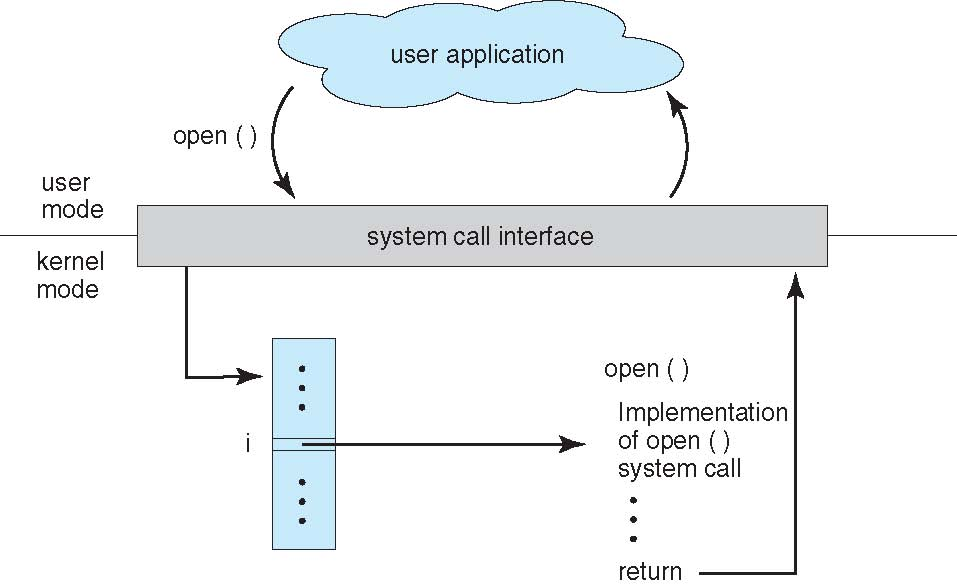
\includegraphics[width=0.7\textwidth]{system-call-interface}
		\caption{System call interface between the application and the OS}
		\label{fig:introduction:system-call}
	\end{figure}

& \textbf{Timer chip:} Component in hardware which prevents users from accessing resources for too long
	&& Process:
		&&& OS sets a millisecond timer before providing control to a user program
		&&& When the period expires, the timer chip sends an interrupt
		&&& CPU decides whether to grant more time or terminate the program

\end{easylist}
\subsection{Structure of an OS}
	\label{subsec:introduction:structure}
\begin{easylist}

& Startup/boot:
	&& OS must be available to hardware when starting
	&& Process:
		&&& Instruction register is loaded with a predefined memory location which is the address of the bootstrap loader in ROM
		&&& Bootstrap loader performs diagnostic tests (Power-on Self Testing)
		&&& From a fixed file location on the disk (the boot block), code is loaded into memory
		&&& Remainder of the loader is loaded
		&&& Kernel is loaded

& \textbf{Simple/monolithic structure:} OS compositional design where the entire system is a single component with no access controls
	&& Used by UNIX in the past
	&& Pro: Efficient if constructed well
	&& Con: Difficult to implement and maintain
	&& For an example diagram, see figure~\ref{fig:introduction:structure-monolithic}
	\begin{figure}[!htb]
		\centering
		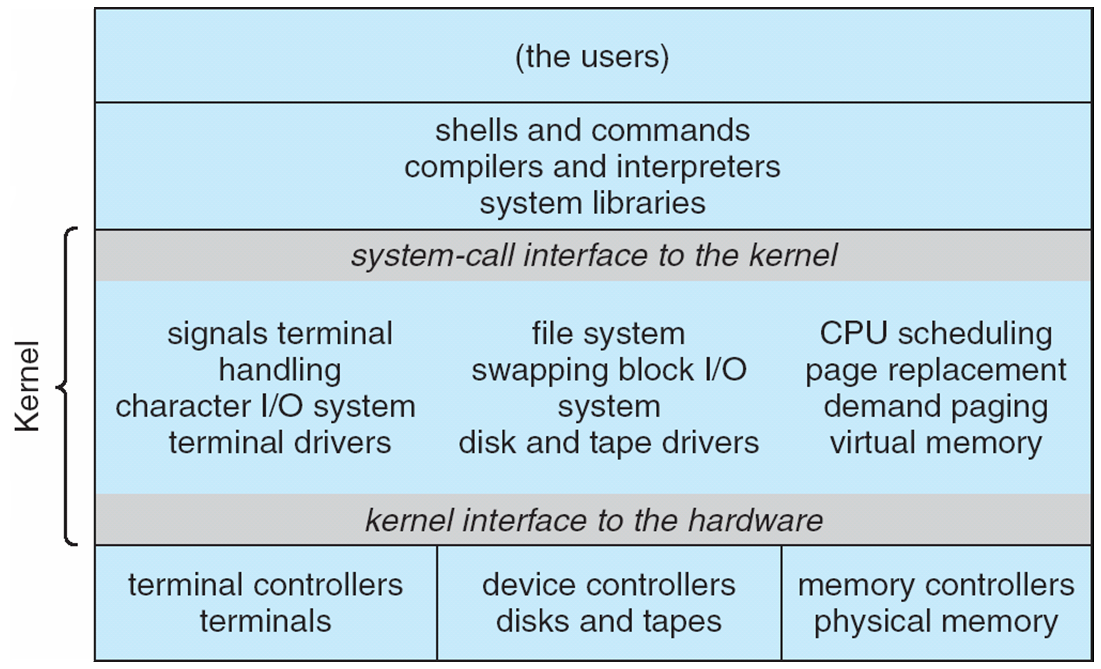
\includegraphics[width=0.6\textwidth]{structure-monolithic}
		\caption{Monolithic structure}
		\label{fig:introduction:structure-monolithic}
	\end{figure}

& \textbf{Layered structure:} OS compositional design where the system is divided into layers, each of which only communicates with the layer directly beneath it
	&& Pro: More reliable than a monolithic structure due to better modularization
	&& Con: Less performant than a monolithic structure due to more switching between handlers
	&& For an example diagram, see figure~\ref{fig:introduction:structure-layered}
	\begin{figure}[!htb]
		\centering
		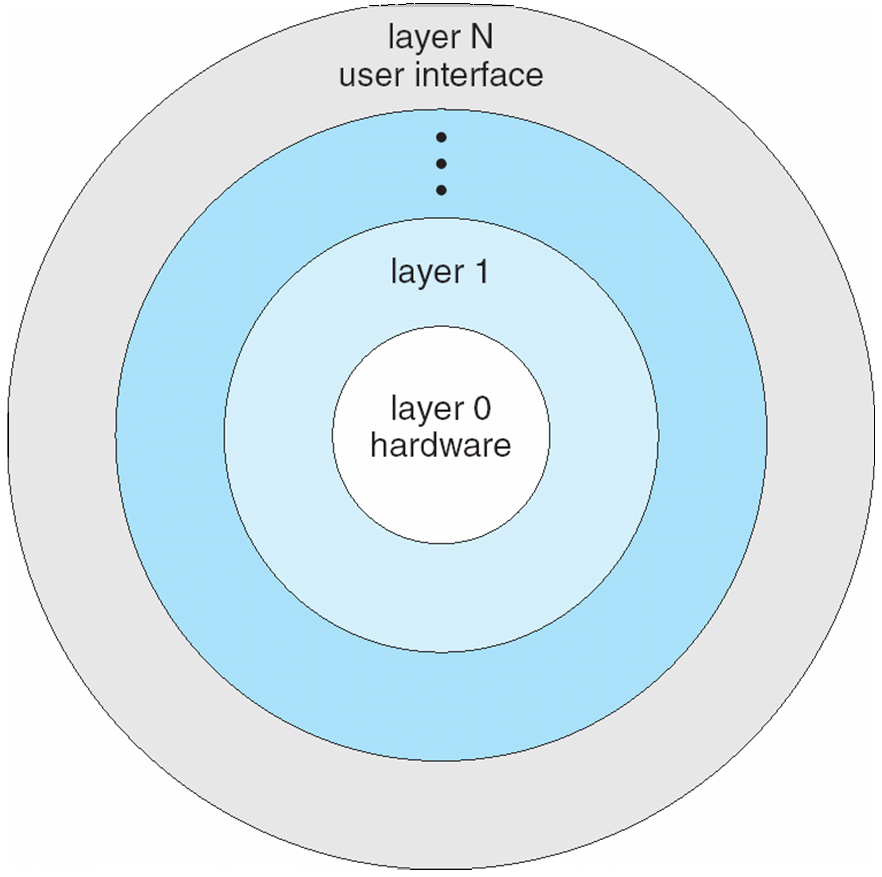
\includegraphics[width=0.5\textwidth]{structure-layered}
		\caption{Layered structure}
		\label{fig:introduction:structure-layered}
	\end{figure}

& \textbf{Microkernel structure:} OS compositional design where user programs only communicate with hardware through the kernel when necessary
	&& \textbf{Interprocess communication:} Kernel passes messages between modules
	&& Pros: Easier to extend and port to new architectures, more secure due to services being isolated to user mode
	&& Cons: Less performant due to indirect communication
	&& For an example diagram, see figure~\ref{fig:introduction:structure-microkernel}
	\begin{figure}[!htb]
		\centering
		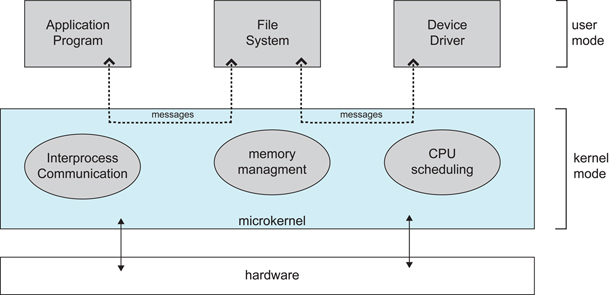
\includegraphics[width=0.8\textwidth]{structure-microkernel}
		\caption{Microkernel structure}
		\label{fig:introduction:structure-microkernel}
	\end{figure}

& \textbf{Modular structure:} OS compositional design where the system is comprised of independent components
	&& Kernel module contains core components; other modules are linked to the kernel module as needed
	&& Pros:
		&&& No need to recompile all code, only the modules with changes
		&&& Modules communicate using defined interfaces
		&&& Easy to maintain, update, and debug
		&&& More flexible than layers
		&&& More efficient than microkernels due to direct communication between modules
	&& Used by modern OSes such as Solaris, Linux
	&& For an example diagram, see figure~\ref{fig:introduction:structure-modular}
	\begin{figure}[!htb]
		\centering
		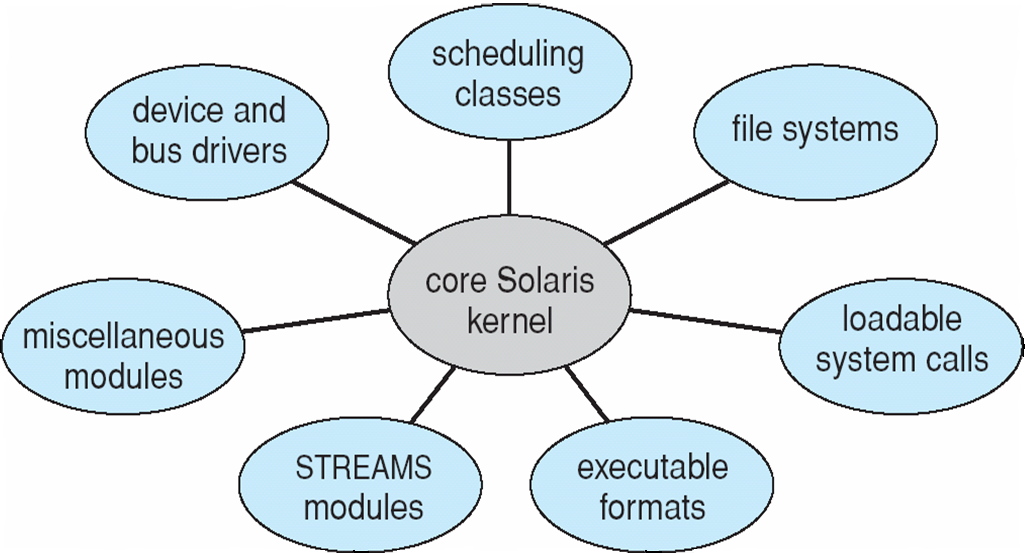
\includegraphics[width=0.7\textwidth]{structure-modular}
		\caption{Modular structure}
		\label{fig:introduction:structure-modular}
	\end{figure}

& \textbf{Hybrid structure:} OS compositional design where the system uses multiple design philosophies
	&& Used by many OSes such as Mac OS X (e.g. has layers and a microkernel, the kernel environment is monolithic, and lower-level drivers are modules)
	&& For an example diagram, see figure~\ref{fig:introduction:structure-hybrid}
	\begin{figure}[!htb]
		\centering
		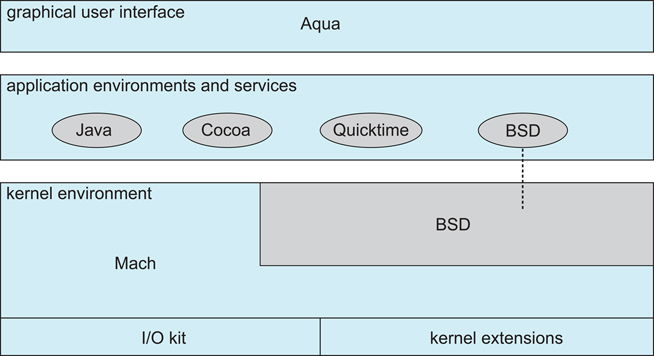
\includegraphics[width=0.7\textwidth]{structure-hybrid}
		\caption{Hybrid structure}
		\label{fig:introduction:structure-hybrid}
	\end{figure}

\end{easylist}
\clearpage